\section{Experimental Setup}\label{sec:experiments}

We evaluate our method on the task shown in Fig. \ref{fig:fig2}, both in simulation and in the real world. This section introduces the details of the experimental setup and provides an overview of the experiments.

\subsection{Simulated Environment}
We use MuJoCo~\citep{todorov12mujoco}, a full-featured simulator for model-based optimization considering body contacts, to evaluate our method in simulation.
This environment consists of a simulated Sawyer robot arm with seven degrees of freedom and a parallel gripper. 
We command the robot with a Cartesian-space position controller.
%% Cut for space
% Two blocks each with 3-DOF and one angled corner on the top are placed on a defined platform on the table in front of the robot. 
% To allow block insertion between the standing blocks, a sufficiently large gap is defined (this gap represents the goal position). 
% Both standing blocks can slide in $x$- and $y$-direction and topple around the $y$-axis.
% The agent receives the end effector position, the end effector forces and torques in relation to the $x$-, $y$- and $z$-axes, all block positions, and the goal position as the observation. In the robot's initial position one block for the insertion process is already picked up by the gripper claws and the gripper is located above the blocks on the tabletop. 

% We use a reward function 
%     \begin{align}
%         r_t = - \|x_g - x_t \|_2 - \lambda (\|\theta_{l} \|_1 + \|\theta_{r} \|_1)
%     \end{align}
% where $x_t$ is the current block position, $x_g$ is the goal position, $\theta_{l}$, $\theta_{r}$ are the angles with respect to the table (in the y-axis) of the left and right blocks, respectively. $\lambda$ is a hyperparameter. 


\subsection{Real-World Environment}
The real-world environment is largely the same as the simulated environment, except for the controller, rewards, and observations.
We command the robot with a compliant joint-space impedance controller we have developed to be smooth and tolerant of contacts.
The positioning of the block being inserted is similar to the simulation but the observation is estimated from a camera-based tracking system as we do not have access to ground truth position information.
%% Cut for space
% Due to the blocks' slight weight and their capability of sliding in the plane ($x$, $y$), the Sawyer is not able to measure contact forces regarding these axes.
% Therefore, we only add the end effector forces in $z$-direction to the observation space instead of observing the end effector forces and torques regarding to the $x$-, $y$- and $z$-axes.
% The reward function was slightly different, being defined as: 
%     \begin{align}
%     \begin{split}
%     r_t = - \|x_g - x_t \|_2 - \lambda (\|\theta_{l} \|_1 + \|\theta_{r} \|_1) \\ - \mu \|X_g - X_t \|_2 - \beta (\|\phi_{l} \|_1 + \|\phi_{r} \|_1)
%     \end{split}
%     \end{align}
% where $x_t$ is the current end effector position, $x_g$ is the goal position, $X_t$ describes the current position of both standing blocks, $X_g$ their desired positions, $\theta_{l}$, $\theta_{r}$ are the angles of the current orientation with respect to the table (in the y-axis) and $\phi_{l}$ and $\phi_{r}$ are the angles of the current orientation with respect to the z-axis of the left and the right block respectively $\lambda$, $\mu$, and $\beta$ are hyperparameters. 

%
% \subsection{Training Details}

\footnotetext{In all simulation plots, we use 10 random seeds and report a $95\%$ confidence interval for the mean.}

\subsection{Overview of Experiments}
%%SL.12.01: This feels like it belongs in the next section
%
In our experiments we evaluate the following research questions:
\begin{enumerate}
    \item Does incorporating a hand-designed controller improve the performance and sample-efficiency of RL algorithms, while still being able to recover from an imperfect hand-designed controller?
    \item Can our method allow robots to be more tolerant of variation in the environment?
    \item Can our method successfully control noisy systems, compared to classical control methods?
\end{enumerate}

\section{Experiments}

\subsection{Sample Efficiency of Residual RL}
In this section, we compare our residual RL method with the human controller alone and RL alone. The following methods are compared:
\begin{enumerate}
    \item Only RL: using the same underlying RL algorithm as our method but without adding a hand-engineered policy
    \item Residual RL: our method which trains a superposition of the hand-engineered controller and a neural network policy, with RL
\end{enumerate}

\subsection{Effect of Environment Variation}
In automation, environments can be subject to noise and solving manufacturing tasks become more difficult as variability in the environment increases. 
It is difficult to manually design feedback controllers that are robust to environment variation, as it might require significant human expertise and tuning. In this experiment, we vary the initial orientation of the blocks during each episode and demonstrate that residual RL can still solve the task. We compare its performance to that of the hand-engineered controller.

To introduce variability in simulation, on every reset we sampled the rotation of each block independently from a uniform distribution $U[-r, r], r \in \{0, 0.05, 0.1, 0.15, 0.2, 0.25, 0.3\}$.

Similarly, in the real world experiments, on every reset we randomly rotated each block to one of three orientations: straight, tilted clockwise, or tilted counterclockwise (tilt was $\pm$  $20^{\circ}$ from original position).

\subsection{Recovering from Control Noise}

Due to a host of issues, such as defective hardware or poorly tuned controller parameters, feedback controllers might have induced noise. Conventional feedback control policies are determined a priori and do not adapt their behavior from data.
However, RL methods are known for their ability to cope with shifting noise distributions and are capable of recovering from such issues.

\begin{figure}[ht!]
    \vspace{6pt}
    \centering
    \begin{subfigure}[b]{0.38\linewidth}
    \renewcommand{\arraystretch}{1.5}
    \footnotesize
        \begin{tabular}{ | c || c | c |}
            \hline
            Misaligned? & No & Yes  \\ \hline
            Residual RL & 20/20 & 15/20  \\ \hline
            Hand-engineered  & 20/20 & 2/20  \\ \hline
        \end{tabular}
        \vspace{.8cm} \\
        \centering
        \normalsize{(a)}
    \end{subfigure}
    \begin{subfigure}[b]{0.3\linewidth}
        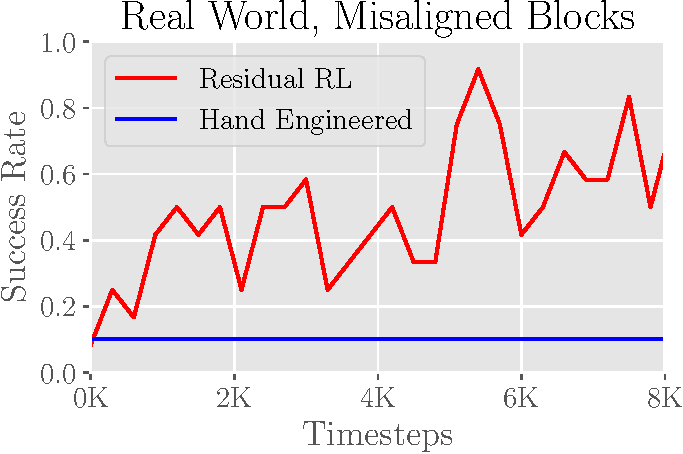
\includegraphics[width=0.99\linewidth]{residualrl/figs/real_world_envvar_success.pdf} \\
        \centering
        (b)
    \end{subfigure}
    \begin{subfigure}[b]{0.3\linewidth}
        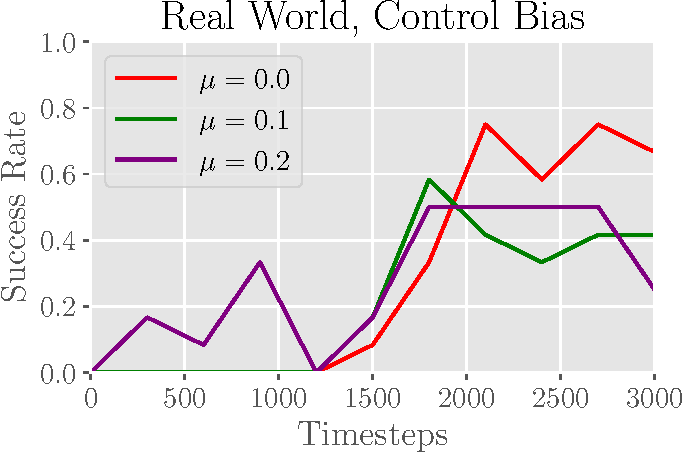
\includegraphics[width=0.99\linewidth]{residualrl/figs/real_world_control_bias.pdf} \\
        \centering
        (c)
    \end{subfigure}
    \vspace{0cm}
    \caption{Outcome of our residual RL method in different experiments during the block assembly task in the real-world. Success rate is recorded manually by human judgment of whether the blocks stayed upright and ended in the correct position. Plot (a) compares the insertion success of residual RL and hand-designed controller depending on the block orientation during run time. Plot (b) shows the success rate of the insertion process during training, where on every reset the blocks are randomly rotated: straight, tilted clockwise, or tilted counterclockwise ($\pm$  $20^{\circ}$) and plot (c) shows the increasing success rate of our method for biased controllers as well even as control bias increases.}%
    \label{fig:environment_variation}
\end{figure}

In this experiment, we introduce a control noise, including biased control noise, and demonstrate that residual RL can still successfully solve the task, while a hand-engineered controller cannot. The control noise follows a normal distribution and is added to the control output of the system at every step:
\begin{align}
    u'_t = u_t + \mathcal{N}(\mu, \sigma^2)
\end{align}

To test tolerance to control noise, we set $\mu = 0$ and vary $\sigma \in [0.01, 0.1]$. In theory, RL could adapt to a noisy controller by learning more robust solutions to the task which are less sensitive to perturbations.

Furthermore, to test tolerance to a biased controller, we set $\sigma = 0.05$ and vary $\mu \in [0, 0.2]$. To optimize the task reward, RL can learn to simply counteract the bias. 

\subsection{Sim-to-Real with Residual RL}

As an alternative to analytic solutions of real-world control problems, we can often instead model the forward dynamics of the problem (ie. a simulator). With access to such a model, we can first find a solution to the problem with our possibly inaccurate model, and then use residual RL to find a realistic control solution in the real world.

In this experiment, we attempt the block insertion task with the side blocks fixed in place. The hand-engineered policy $\pi_\text{H}$ in this case comes from training a parametric policy in simulation of the same scenario (with deep RL). We then use this policy as initialization for residual RL in the real world.